\documentclass[10pt, compress]{beamer}
\usetheme{m}
\usepackage{booktabs}
\usepackage[ampersand]{easylist}
\usepackage{minted}
\usemintedstyle{manni}
\usepgfplotslibrary{dateplot}

\title{Satellid: Personal Knowledge Manager}
\subtitle{with Web Technologies}
\date{18 March 2015}
\author{Muhammad Haidar Hanif}
\institute{Informatics Engineering - Gunadarma University}

\begin{document}

% ============================================================

\maketitle

% ============================================================

\begin{frame}[fragile]
  \frametitle{Outline}

  \begin{description}
    \item[Introduction]
    \item[Literature Study]
    \item[Analysis \& Design]
    \item[Implementation \& Testing]
    \item[Conclusion \& Suggestion]
  \end{description}

\end{frame}

% ============================================================

\section{Introduction}

% ------------------------------------------------------------

\begin{frame}[fragile]

  \begin{center}
  There are tons of \alert{daily personal knowledge} that must be managed,
  but they can't be handled with regular tools.
  \end{center}

\end{frame}

% ------------------------------------------------------------

\begin{frame}[fragile]
  \centering

  \alert{Daily personal knowledge} are things like details or facts of:

  \begin{figure}[ht]
    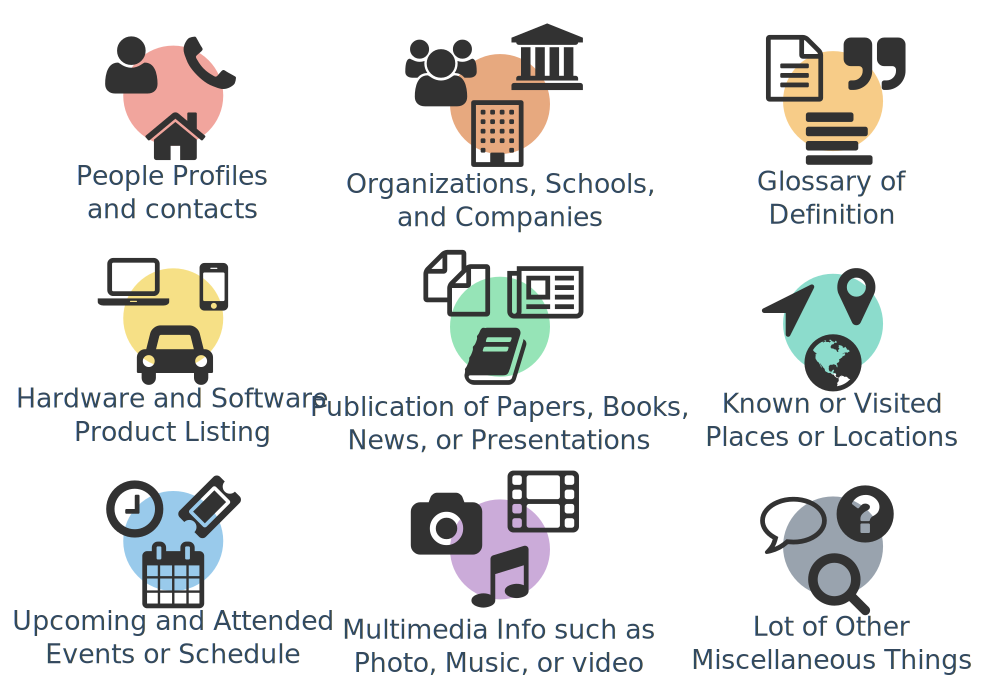
\includegraphics[width=10cm]{include/knowledge-daily.png}
  \end{figure}

  All of these are also the \alert{context of knowledge}

\end{frame}

% ------------------------------------------------------------

\begin{frame}[fragile]
  \centering

  There are a \alert{lot of tools/systems} for each, that contains knowledge
  %Most of them also only available when online.

  \begin{figure}[ht]
    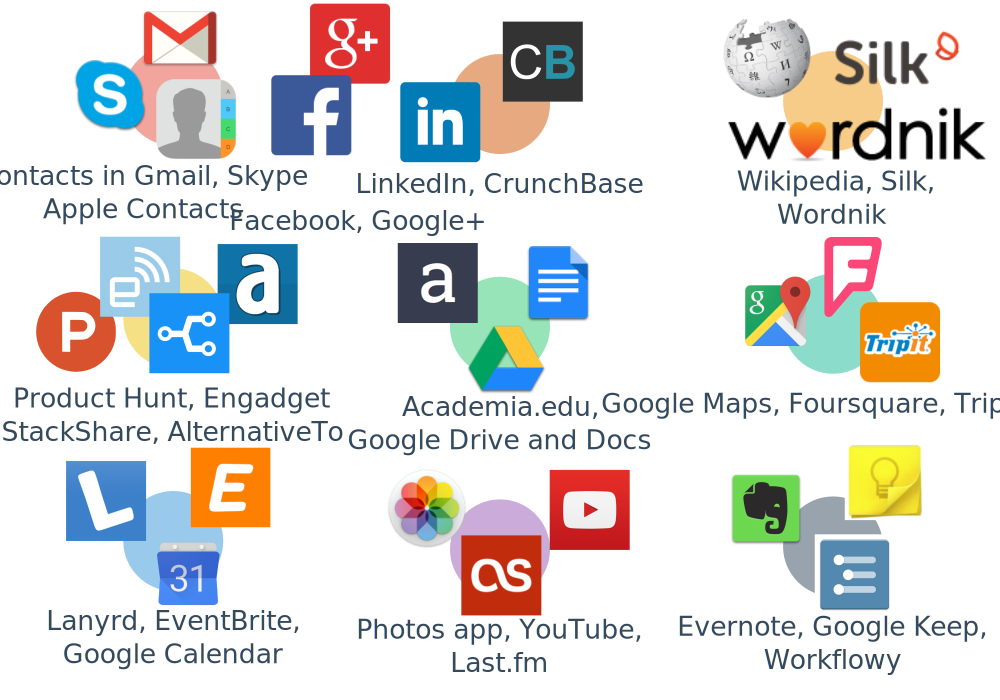
\includegraphics[width=10cm]{include/knowledge-tools.png}
  \end{figure}

  There is a \alert{need for a single personalized system}

\end{frame}

% ------------------------------------------------------------

\begin{frame}[fragile]
  \centering

  How to manage those \alert{daily personal knowledge} with \alert{single system}?
  % So how to manage those tons of daily personal knowledge we have with just a simple and single system of knowledge manager that implemented with Web technologies?

\end{frame}

% ------------------------------------------------------------

\begin{frame}[fragile]
  \frametitle{Primary Background}

  \begin{itemize} \itemsep0pt
    \item Solve a problem around \alert{daily knowledge management} \\
          with a system that is personal.
    \item Essential knowledge are mostly separated into too many softwares.
    \item Need for a simple and single personalized system.
    \item Managing knowledge should use a knowledge manager.
  \end{itemize}

\end{frame}

% ------------------------------------------------------------

\begin{frame}[fragile]
  \frametitle{Primary Objective}

  Define and develop a personal knowledge manager named \alert{``Satellid''},\\
  that built using Web technologies.
  % utilize knowledge template which use context and structure, to store and managing personal daily knowledge.

\end{frame}

% ------------------------------------------------------------

\begin{frame}[fragile]
  \frametitle{Problem Definition}

  \begin{enumerate}
    \item How to manage tons of personal knowledge with just a simple and single system of knowledge manager?
    \item How can knowledge manager naturally structure the data into knowledge that has context?
  \end{enumerate}

\end{frame}

% ------------------------------------------------------------

\begin{frame}[fragile]
  \frametitle{Problem Scope}

  \begin{itemize} \itemsep0pt
    \item Create a \alert{simple system} to do \alert{daily knowledge management} for \alert{personal} use
    % with \alert{basic \textsc{browse, read, edit, add, delete} (BREAD) features}.
    \item The main methodologies are \alert{agile}, \alert{MVP}, and \alert{ATDD}.
    \item The main technologies are \alert{MongoDB}, \alert{JavaScript}, and \alert{Meteor framework}.
  \end{itemize}

\end{frame}

% ============================================================

\section{Literature Study}

% ------------------------------------------------------------

\begin{frame}[fragile]
  \frametitle{Knowledge Management System}
  \centering

  \begin{figure}[ht]
    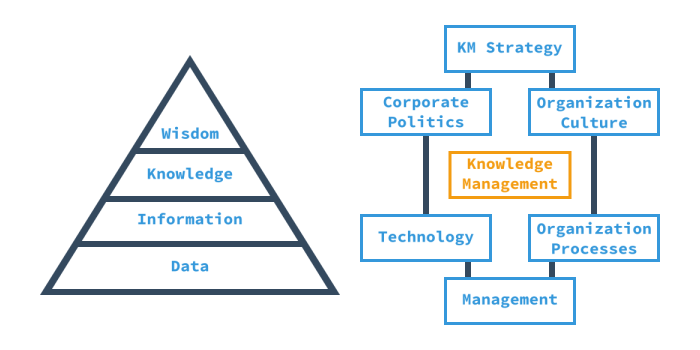
\includegraphics[width=8cm]{include/literature-kms.png}
  \end{figure}

  Data-Information-Knowledge-Wisdom (\alert{DIKW}),\\
  Knowledge Management System (\alert{KMS}),\\
  \alert{Personal Knowledge Manager}

\end{frame}

% ------------------------------------------------------------

\begin{frame}[fragile]
  \frametitle{Software Development Life Cycle (SDLC)}
  \centering

  \begin{figure}[ht]
    \vspace{-1cm}
    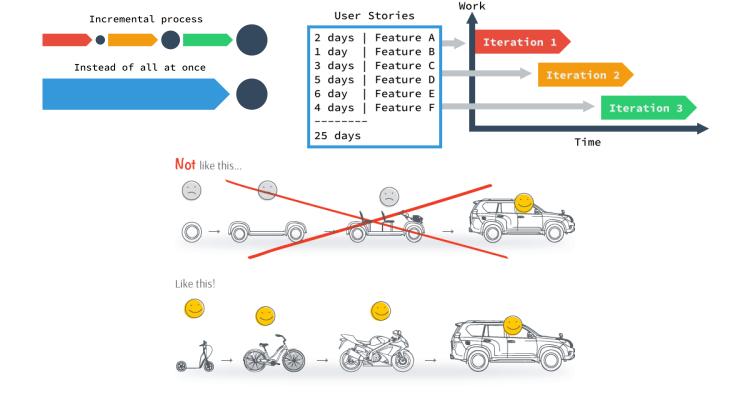
\includegraphics[width=11cm]{include/literature-sdlc.png}
  \end{figure}

  \alert{Agile} methodologies,\\
  Minimum Viable Product (\alert{MVP})\\
  %Acceptance Test Driven Development (\alert{ATDD})

\end{frame}

% ------------------------------------------------------------

\begin{frame}[fragile]
  \frametitle{Design Pattern}
  \centering

  \begin{figure}[ht]
    \vspace{-1cm}
    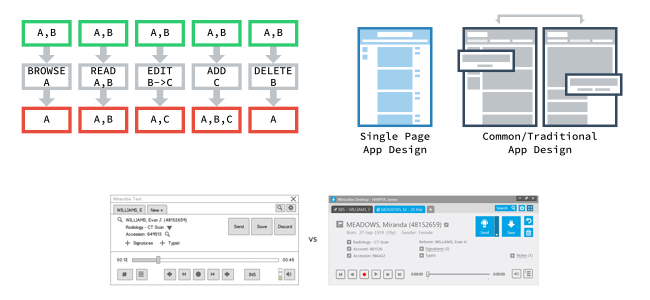
\includegraphics[width=11cm]{include/literature-design-pattern.png}
  \end{figure}

  \textsc{browse, read, edit, add, delete} (\alert{BREAD}),\\
  simple interaction and interface design with \alert{mockup},\\
  Single Page Application (\alert{SPA})

\end{frame}

% ------------------------------------------------------------

\begin{frame}[fragile]
  \frametitle{Database}
  \centering

  \begin{figure}[ht]
    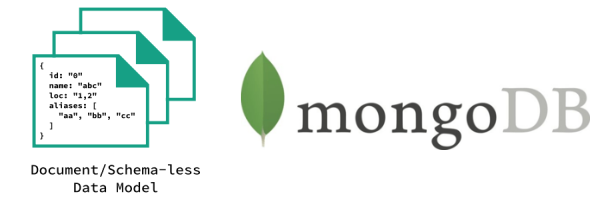
\includegraphics[width=8cm]{include/literature-database.png}
  \end{figure}

  Document-based \alert{NoSQL} database named \alert{MongoDB}

\end{frame}

% ------------------------------------------------------------

\begin{frame}[fragile]
  \frametitle{Programming}
  \centering

  \begin{figure}[ht]
    
\includegraphics[width=8cm]{include/literature-programming.png}
  \end{figure}

  With \alert{JavaScript} and \alert{JSON} related technologies

\end{frame}

% ------------------------------------------------------------

\begin{frame}[fragile]
  \frametitle{Platform}
  \centering

  \begin{figure}[ht]
    
\includegraphics[width=8cm]{include/literature-platform.png}
  \end{figure}

  on top of \alert{Node.js}

\end{frame}

% ------------------------------------------------------------

\begin{frame}[fragile]
  \frametitle{Web Application}
  \centering

  \begin{figure}[ht]
    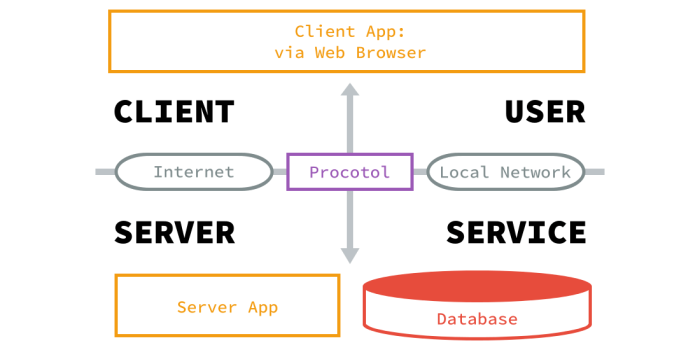
\includegraphics[width=8cm]{include/literature-webapp.png}
  \end{figure}

  build a \alert{Web application}\\
  %with general web application architecture

\end{frame}

% ------------------------------------------------------------

\begin{frame}[fragile]
  \frametitle{Framework}
  \centering

  \begin{figure}[ht]
    
\includegraphics[width=8cm]{include/literature-framework.png}
  \end{figure}

  using \alert{full stack framework} named \alert{Meteor}
  % full stack = frontend + backend

\end{frame}

% ------------------------------------------------------------

\begin{frame}[fragile]
  \frametitle{Software Testing}
  \centering

  \begin{figure}[ht]
    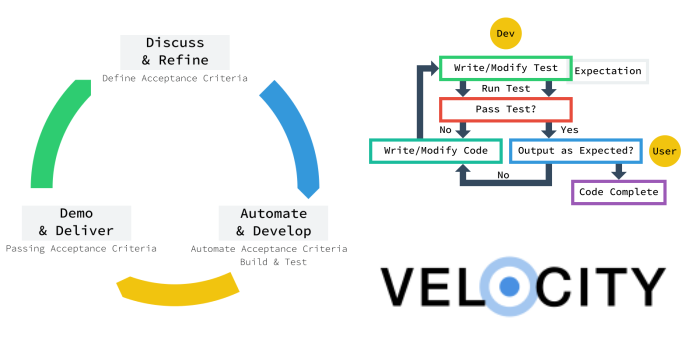
\includegraphics[width=8cm]{include/literature-testing.png}
  \end{figure}

  \alert{software tested} in Acceptance Test Driven Development (\alert{ATDD})

\end{frame}

% ------------------------------------------------------------

\begin{frame}[fragile]
  \frametitle{Source Code Management}
  \centering

  \begin{figure}[ht]
    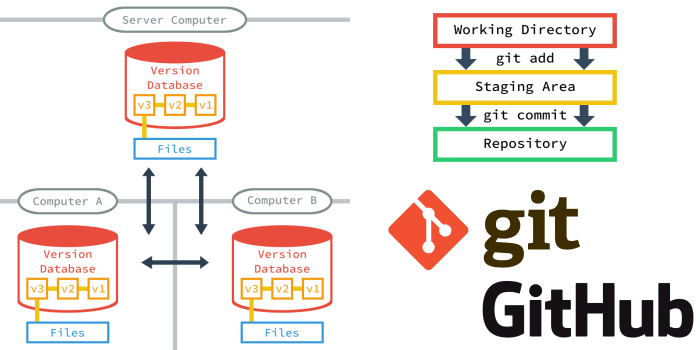
\includegraphics[width=8cm]{include/literature-scm.png}
  \end{figure}

  source code is version controlled using \alert{Git}\\
  and distributed via \alert{GitHub}

\end{frame}

% ============================================================

\section{Analysis \& Design}

% ------------------------------------------------------------

\begin{frame}[fragile]
  \frametitle{Analysis}

    \begin{block}{Target User:}
      Person who frequently gather and really want to manage their tons of knowledge at almost everytime
    \end{block}

\end{frame}

% ------------------------------------------------------------

\begin{frame}[fragile]
  \frametitle{Analysis}

  \begin{figure}[ht]
    \includegraphics[width=10cm]{include/users/types.jpg}
  \end{figure}

  \begin{block}{User Types:}
    Regular person, researcher, engineer, developer, designer,\\
    information architect, event speaker, student, teacher,\\
    leader, collaborator, colleagues, recruiter, etc
  \end{block}

\end{frame}

% ------------------------------------------------------------

\begin{frame}[fragile]
  \frametitle{Design: Contextual System}
  \centering

  \begin{figure}[ht]
    \centering
    \includegraphics[width=9cm]{include/satellid-contextual.png}
    \label{fig:satellid-contextual}
  \end{figure}

  A data and template approach to classify the knowledge with its context and structure.

\end{frame}

% ------------------------------------------------------------

\begin{frame}[fragile]
  \frametitle{Design: Application Architecture}

  \begin{figure}[ht]
    \centering
    \vspace{-25pt}
    \includegraphics[height=8.5cm]{include/satellid-app-arch.png}
    \vspace{-10pt}
    \caption{Application Architecture}
    \label{fig:satellid-app-arch}
  \end{figure}

\end{frame}

% ------------------------------------------------------------

\begin{frame}[fragile]
  \frametitle{Design: User Interface Mockup}

  \begin{figure}[ht]
    \centering
    \vspace{-25pt}
    \includegraphics[height=8.5cm]{include/satellid-app-ui.png}
    \vspace{-10pt}
    \caption{User Interface Mockup Design}
    \label{fig:satellid-app-ui}
  \end{figure}

\end{frame}

% ------------------------------------------------------------

\begin{frame}[fragile]
  \frametitle{Design: User Interaction}

  \begin{figure}[ht]
    \centering
    \vspace{-25pt}
    \includegraphics[height=8.5cm]{include/satellid-app-uix.png}
    \vspace{-10pt}
    \caption{User Interaction Design}
    \label{fig:satellid-app-uix}
  \end{figure}

\end{frame}

% ============================================================

\section{Implementation \& Testing}

% ------------------------------------------------------------

\begin{frame}[fragile]
  \frametitle{Implementation: Code}

  Snippets of Server Code
  \begin{minted}[fontsize=\small]{javascript}
    if (Meteor.isServer) {
      Meteor.startup(function() {
        // ...
      });
    }
  \end{minted}

  Snippets of Client Code
  \begin{minted}[fontsize=\small]{javascript}
    if (Meteor.isClient) {
      Template.add.events({
        "click": function() {
          // ...
        }
      });
    }
  \end{minted}

\end{frame}

% ------------------------------------------------------------

\begin{frame}[fragile]
  \frametitle{App Result Screenshots: READ}

  \begin{figure}[ht]
    \centering
    \vspace{-1cm}
    \includegraphics[height=10cm]{include/satellid-app-results_read.png}
    \vspace{-10pt}
    \label{fig:satellid-app-results_read}
  \end{figure}

\end{frame}

% ------------------------------------------------------------

\begin{frame}[fragile]
  \frametitle{App Result Screenshots: BROWSE}

  \begin{figure}[ht]
    \centering
    \vspace{-1cm}
    \includegraphics[height=10cm]{include/satellid-app-results_browse.png}
    \vspace{-10pt}
    \label{fig:satellid-app-results_browse}
  \end{figure}

\end{frame}

% ------------------------------------------------------------

\begin{frame}[fragile]
  \frametitle{App Result Screenshots: ADD}

  \begin{figure}[ht]
    \centering
    \vspace{-1cm}
    \includegraphics[height=10cm]{include/satellid-app-results_add.png}
    \vspace{-10pt}
    \label{fig:satellid-app-results_add}
  \end{figure}

\end{frame}

% ------------------------------------------------------------

\begin{frame}[fragile]
  \frametitle{App Result Screenshots: EDIT}

  \begin{figure}[ht]
    \centering
    \vspace{-1cm}
    \includegraphics[height=10cm]{include/satellid-app-results_edit.png}
    \label{fig:satellid-app-results_edit}
  \end{figure}

\end{frame}

% ------------------------------------------------------------

\begin{frame}[fragile]
  \frametitle{App Result Screenshots: DELETE}

  \begin{figure}[ht]
    \centering
    \vspace{-1cm}
    \includegraphics[height=10cm]{include/satellid-app-results_delete.png}
    \vspace{-10pt}
    \label{fig:satellid-app-results_delete}
  \end{figure}

\end{frame}

% ============================================================

\section{Closing}

% ------------------------------------------------------------

\begin{frame}[fragile]
  \frametitle{Conclusion}

  Simple and \alert{single system} of managing tons of \alert{personal daily knowledge}
  that implemented with \alert{Web technologies}

\end{frame}

% ------------------------------------------------------------

\begin{frame}[fragile]
  \frametitle{Suggestion for Future Work}

  \begin{itemize} \itemsep0pt
    \item More predefined context and field.
    \item Can have custom form
    \item Can easily import and export, including backup
    \item \textsc{BREAD} a template
    \item Multimedia support
    \item Integration with other networks
    % User start to use the app with a blank state, need to add all their present knowledge manually along the time.
  \end{itemize}

\end{frame}

% ============================================================

\plain{Thank You}

% ============================================================

\plain{Extra Notes}

% ------------------------------------------------------------

\begin{frame}[fragile]
  \frametitle{Satellid}

  \begin{figure}[ht]
    \centering
    \vspace{-1cm}
    %TODO\includegraphics[width=10cm]{include/satellite.jpg}
    \label{fig:satellite}
  \end{figure}

\end{frame}

% ------------------------------------------------------------

\begin{frame}[fragile]
  \frametitle{Agile User Stories}

  \begin{enumerate} \itemsep0pt
    \item As a System, I need to be run on supported platform and via a network
    \item As a System, I can have the data imported without the app opened
    \item As a User, I want to use the app via web browser
    \item As a User, I want to read knowledge that already stored
    \item As a User, I want to search a knowledge and view the search result
    \item As a User, I want to add a new knowledge based on context
    \item As a User, I want to delete a stored knowledge
    \item As a User, I want to edit a stored knowledge
  \end{enumerate}

\end{frame}

% ------------------------------------------------------------

\begin{frame}[fragile]
  \frametitle{Example of Feature File}

  \begin{minted}[fontsize=\small]{ruby}
    Feature: Example feature title

      As a user of this feature
      I want to have these steps
      So that I can have the expected result

      Scenario: Specific situation description
        Given a condition
        And an other condition
        When a performed action by someone
        Then an output is presented
  \end{minted}

\end{frame}

% ------------------------------------------------------------

\begin{frame}[fragile]
  \frametitle{Testing Result with Velocity}

  \begin{figure}[ht]
    \centering
    \vspace{-25pt}
    \includegraphics[height=8.5cm]{include/satellid-app-test.png}
    \vspace{-10pt}
    \label{fig:satellid-app-test}
  \end{figure}

\end{frame}

% ------------------------------------------------------------

\begin{frame}[fragile]
  \frametitle{SQL vs Document-based (NoSQL)}

  \begin{figure}[ht]
    \centering
    \vspace{-25pt}
    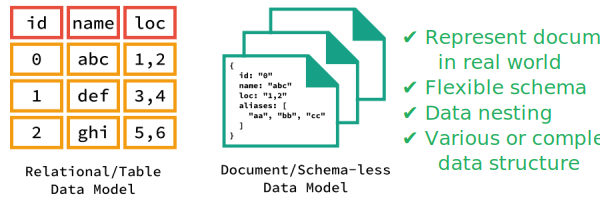
\includegraphics[width=11cm]{include/literature-nosql.png}
    \vspace{-10pt}
    \label{fig:literature-nosql}
  \end{figure}

\end{frame}

% ============================================================

\plain{Extra Notes}

% ============================================================

\end{document}
